\documentclass[a4paper]{oblivoir}
\usepackage{amsmath,amssymb,kotex,kswrapfig,mdframed,paralist}
\usepackage{fapapersize}
\usefapapersize{210mm,297mm,10mm,*,10mm,*}

\usepackage{tabto,pifont}
\TabPositions{0.2\textwidth,0.4\textwidth,0.6\textwidth,0.8\textwidth}
\newcommand\tabb[5]{\par\noindent
\ding{172}\:{\ensuremath{#1}}
\tab\ding{173}\:\:{\ensuremath{#2}}
\tab\ding{174}\:\:{\ensuremath{#3}}
\tab\ding{175}\:\:{\ensuremath{#4}}
\tab\ding{176}\:\:{\ensuremath{#5}}}

\usepackage{graphicx}

%\pagestyle{empty}

%%% Counters
\newcounter{num}

%%% Commands
\newcommand\prob[1]
{\vs\bigskip\par\noindent\stepcounter{num} \textbf{문제 \thenum) #1}\par\noindent}

\newcommand\pb[1]{\ensuremath{\fbox{\phantom{#1}}}}

\newcommand\ba{\ensuremath{\:|\:}}

\newcommand\vs[1]{\vspace{70pt}}

\newcommand\an[1]{\bigskip\par\noindent\textbf{문제 #1)}\par\noindent}

%%% Meta Commands
\let\oldsection\section
\renewcommand\section{\clearpage\oldsection}

\let\emph\textsf

\begin{document}
\begin{center}
\LARGE종현, 추가과제 02
\end{center}
\begin{flushright}
날짜 : 2017년 \(\pb3\)월 \(\pb{10}\)일 \(\pb{월}\)요일
,\qquad
제한시간 : \pb{17년}분
,\qquad
점수 : \pb{20} / \pb{20}
\end{flushright}

%
\prob{}
다음 물음에 답하여라.
\begin{enumerate}[(1)]
\item
\(_{20}C_{r^2+1}=_{20}C_{r-1}\)을 만족하는 자연수 \(r\)의 값을 구하여라.
\item
\(1\le r<n\)일 때, \(_nC_r=_{n-1}C_{r-1}+_{n-1}C_{r}\)가 성립함을 보여라.
\end{enumerate}

%
\prob{}
남자 \(6\)명, 여자 \(4\)명이 있다.
\begin{enumerate}[(1)]
\item
이 중에서 남자 \(3\)명, 여자 \(4\)명을 뽑는 경우는 몇 가지인가?
\item
이 중에서 \(6\)명을 뽑을 때, 여자 \(4\)명이 포함된 경우는 몇 가지인가?
\item
이 중에서 \(4\)명을 뽑을 때, 적어도 여자 \(1\)명이 포함되는 경우는 몇 가지인가?
\item
이 중에서 \(4\)명을 뽑을 때, 적어도 남녀 \(1\)명씩이 포함되는 경우는 몇 가지인가?
\end{enumerate}

%
\prob{}
남학생 \(5\)명, 여학생 \(4\)명 중에서 남학생 \(3\)명, 여학생 \(2\)명을 뽑아서 다음 방법으로 앉힐 때, 그 경우의 수를 구하여라.
\begin{enumerate}[(1)]
\item
일렬로 앉힌다.
\item
원탁에 앉힌다.
\item
남학생 준형이와 여학생 소희를 반드시 포함하고, 서로 이웃하게 원탁에 앉힌다.
\end{enumerate}

%
\prob{}
\begin{minipage}{0.45\textwidth}
오른쪽 그림과 같이 좌표평면에 12개의 점이 있다.
다음을 구하여라.
\begin{enumerate}[(1)]
\item
두 점을 연결하는 선분의 개수
\item
두 점을 연결하는 직선의 개수
\item
세 점을 꼭짓점으로 하는 삼각형의 개수
\end{enumerate}
\end{minipage}
\begin{minipage}{0.45\textwidth}
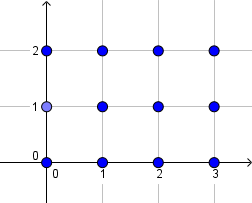
\includegraphics[width=0.5\textwidth]{lattices}
\end{minipage}

%
\prob{}
\begin{minipage}{0.45\textwidth}
오른쪽 그림은 같은 원판의 다섯 곳에 빨강, 노랑, 파랑, 주황, 초록의 5가지 색을 사용하여 인접한 곳은 서로 다른 색을 칠하여 구별하려고 한다.
다음 물음에 답하여라.
\begin{enumerate}[(1)]
\item
5가지 색을 모두 사용하여 칠하는 방법의 수를 구하여라.
\item
5가지 색 중 4가지 색을 사용하여 칠하는 방법의 수를 구하여라.
\end{enumerate}
\end{minipage}
\begin{minipage}{0.45\textwidth}
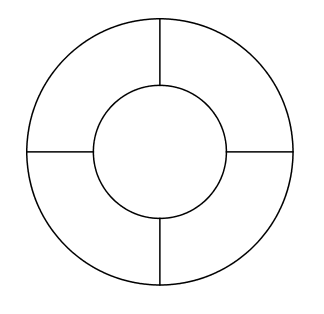
\includegraphics[width=0.5\textwidth]{paint}
\end{minipage}


%
\prob{}
방정식 \(x+y+z+w=10\)에 대하여 다음을 구하여라.
\begin{enumerate}[(1)]
\item
음이 아닌 정수해의 개수
\item
양의 정수해의 개수
\end{enumerate}

%
\prob{}
서로 같은 공 7개를 서로 다른 상자 3개에 나누어 넣으려고 한다.
다음 물음에 답하여라.
\begin{enumerate}[(1)]
\item
빈 상자가 있어도 된다고 할 때, 넣는 방법의 수를 구하여라.
\item
빈 상자가 없도록 넣는 방법의 수를 구하여라.
\item
넣은 공의 개수가 각각 홀수가 되도록 넣는 방법의 수를 구하여라.
\end{enumerate}

%
\prob{}
\(A=\{1,2,3\}\), \(B=\{4,5,6,7\}\)일 때, 함수 \(f:A\to B\) 중 다음 조건을 만족시키는 함수의 개수를 구하여라.
\begin{enumerate}[(1)]
\item
\(i\neq j\)이면 \(f(i)\neq f(j)\)
\item
\(i<j\)이면 \(f(i)<f(j)\)
\item
\(i<j\)이면 \(f(i)\le f(j)\)
\end{enumerate}



\end{document}